\chapter{Spoken Dialogue Systems}
\label{chap:spoken_dialogue_systems}

\lettrine{T}{his} chapter gives an overview on the \aclp{sds}, including common architectures, different system types, and implementation techniques.
The concept of adaptive \aclp{sds}, which is a core idea in this work, is introduced as well, along with the challenges involved and examples of possible adaptation strategies on different levels.

\pagebreak

%\section{What is a spoken dialogue system?}
%\label{sec:what_is_a_sds}
%\todo[inline]{here talk about what is a dialogue, a spoken dialogue, turn, when an interaction becomes a dialogue (is every interaction with a machine is a dialogue system?), etc. can really use the introductions given by Olga in the SDS seminar}

\noindent
\Acfp{sds} offer a wide range of services and are used in various forms every day both for commercial and personal purposes.
The main difference between them and many other ways to communicate with computers is the use of speech -- and mostly speech alone -- for interaction.
This offers benefits to the users, like begin able to perform tasks while keeping their hands free, contrary to systems that require textual input from a keyboard or haptic touch on a screen.
We are witnessing an ever-growing presence of voice-activated devices, like speech-activated cars, hands-free medical assistants, and \acp{its}.
These devices support more and more functionalities in a way that is more comfortable and intuitive for users.
It can be expected that in the near future such devices will be used not only by individuals, but also in more social contexts, including interactions where multiple humans are involved.
This makes the understanding and improvement of social skills in \acp{sds} all the more important.

The common architecture of \acp{sds} is explained in \cref{sec:architecture_sds}, along with details about each component and free tools for building them.
\Cref{sec:types_of_sdss} gives an overview of an application that uses a \ac{sds} to communicate with users.
A roadmap toward \acp{sds} with vocal accommodation capabilities as well as the challenges involved are discussed in \cref{sec:adaptive_spoken_dialogue_systems}.
Such capabilities would improve the personalization and overall experience of the interaction.

\section{Architecture of \aclp{sds}}
\label{sec:architecture_sds}

As shown in \cref{fig:sds_architecture}, the architecture is symmetric in terms of input and output types.
Each cycle starts and ends with speech signals, generated first by the user, and then by the system (a more sophisticated system can also take the initiative).
The content of the utterance, usually referred to as \emph{intent}, is then extracted to determine its objective.
Similarly, the system's speech output is based on generated content that captures some intent.
The \enquote{brain} at the core of the cycle decides what intent is most suitable for the user's input.
This may be done purely by learning from provided dialogue examples, with the help of external information or databases, based on hand-crafted rules, or some combination of those.
This simplified flow assumes that the user and the system take turns alternately, one at a time.
However, one interlocutor may of course needs multiple consecutive turns to convey the message due to length or no response from the other.
Although each component is a whole research area by itself, there are numerous open-source implementations that help to quickly build a basic \ac{e2e} system and focus on a specific one.
Brief overviews of these \ac{nlp} tasks are given in \crefrange{subsec:automatic_speech_recognition}{subsec:text-to-speech_synthesis}.
Note that this is a basic typical architecture and each component may be extended or modified.
Specifically, this architecture changes substantially in fully neural-based systems.
However, even in that case, the general flow (and by extension the training data) remain the same.
%
\begin{figure}[t]
	\centering
	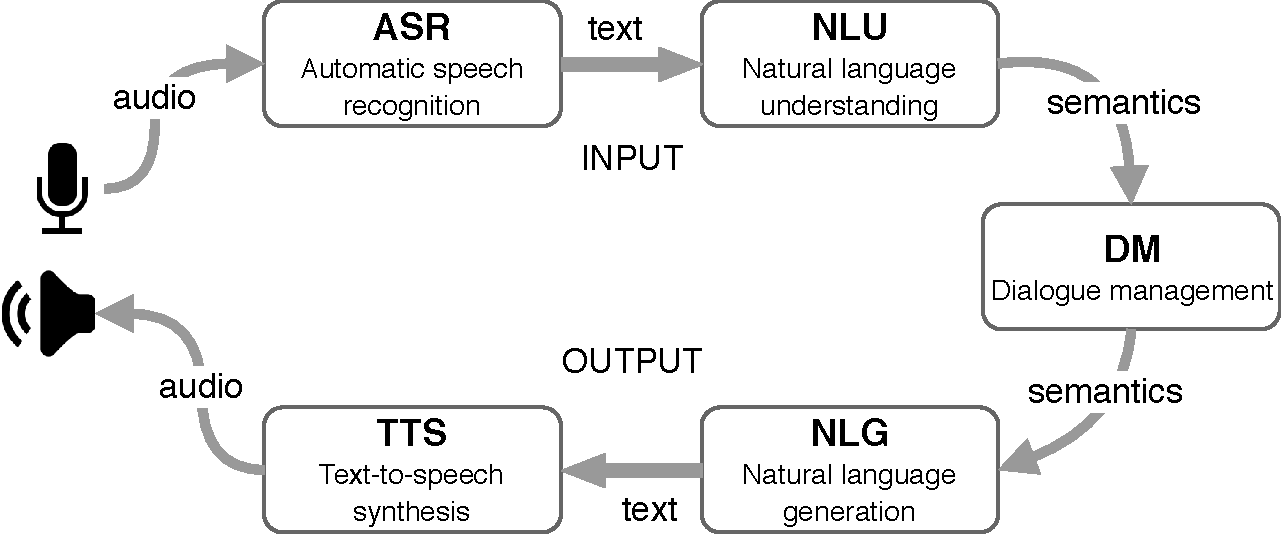
\includegraphics[width=\linewidth]{sds_architecture}
	\caption[Architecture of a spoken dialogue system]
	{A typical architecture of a spoken dialogue system.
	The interaction lifecycle is symmetric, and for each analysis input step there is a corresponding generation output step.
	The exchange usually starts with a user spoken utterance and ends with the system's spoken response.}
	\label{fig:sds_architecture}
\end{figure}

\subsection{\Acl{asr}}
\label{subsec:automatic_speech_recognition}

An essential condition for verbal communication is to be able to hear what the interlocutor says and process it into words.
For computer, this is done using \acf{asr}, which transfers the audio signals produced by the user's articulators into some machine-readable form that can subsequently be fed to the \ac{nlu} component.
This step is crucial for vocal accommodation, as it the only component that accesses the audio signal.
However, \acp{sds} predominantly merely use it to extract the said words and discard it afterwards.
As a result, they know \emph{what} was said by the user (subjected to the quality of the \ac{asr}) but not \emph{how} it was said.
For any kind of responsive behavior, this component must be extended to provide some additional information about the input speech.

\subsubsection{Tools}
\label{subsubsec:tools_asr}

Kaldi \citep{Povey2011kaldi} and CMU Sphinx \citep{Lamere2003sphinx} are free-to-use \ac{asr} engines that offer various functionalities, including training a model on a custom dataset.
For the purpose of vocal accommodation, one benefit of using such modifiable toolkits is the ability to access the phoneme times.
This is crucial for detecting and tracking certain phonetic features, and segmental ones in particular (see \cref{chap:convergence_module_for_sdss} for utilization of this).

\subsection{\Acl{nlu}}
\label{subsec:natural_language_understanding}

After getting the words spoken by the user, the system needs to infer an intention from them, i.e., what the user wants to achieve in this turn.
This is the role of the \acf{nlu} component.
An intention can be as simple as asking the \ac{sds} to perform a task (e.g., to turn on the radio in a voice-activated car).
such requests are mostly recognizable by pre-defined keywords the system can look for in the transcribed input text.
Other requests, like inquiring information about a place or booking a flight, require the system to be able to withdraw -- and properly formulate -- information from some source.
Such tasks require further information (e.g., flight origin and destination, date, price range, etc.) to be completed, or, if said information not provided by the user, additional turns where the system asks for the missing bits.
This process is called slot-filling.
\putref{need example reference for slot filling?}
More complex reactions, and especially in the case of chatbots, demands deeper semantic analysis, as the intention might not be explicitly articulated and in some cases, such a defined intention may not even exist.

%\subsubsection{Tools}
%\label{subsubsec:tools_nlu}

\subsection{\Acl{dm}}
\label{subsec:dialogue_management}

After completing processing the user's input, a decision must be made by the \ac{sds} as to how to react.
This is done by the \acf{dm}, which is the central component of a \ac{sds}.
The \ac{dm} is typically divided into \emph{belief tracker} and \emph{policy} modules.
The former accumulates information regarding the user's wish based on current and previous turns, while the latter is responsible for determining the most appropriate response to that intention.
If any additional data is required for satisfying the user's needs, e.g., some information from the web or a database, the retrieval will be done by the \ac{dm}.
The same goes for specific domain knowledge, which can be made available to the system as part of its implementation.
Deciding on the best action can be achieved using a deterministic rule system for a small number of simple cases (a \ac{cnc} system, for example), but need more sophisticated models for more involved situations.
One commonly used technique is reinforcement learning, which is suitable for making selecting an action based on a given state (the \enquote{environment}).
All these conditions determine how flexible and elaborate the system is, and specifically how large is the domain -- or domains -- it can handle.

\putref{references for rule-based system, RL-based system (Milica?), and adapting DM (add sentence about that at the end)}

\todo[inline]{if it helps, can add a graph like the one from Milica's slide: breadth vs.\ depth of domain in SDS (variety vs.\ complexity). replicate the graph Milica showed in her talk (x-axis is breadth and y-axis depth, with some examples along combinations of the axes.}

%\subsubsection{Tools}
%\label{subsubsec:tools_dm}

\subsection{\Acl{nlg}}
\label{subsec:natural_language_generation}

After deciding on the most appropriate response to the user, the system needs to convey it in a human-understandable manner, namely words.
The process is reversed to \ac{nlg}, i.e., generating text based on a certain intent.
Depending on the user's input intent, the system may respond with simple acknowledgment statements, repetition and information approval, or completely newly formed full sentences.
Additional challenges of this task often root from things that could be reduced or ignored in \ac{nlu}, but must be precise in \ac{nlg}.
For example, using wrong verb conjugations and tenses will cause the system's response to sound ungrammatical or ill-formed in some cases, but could even convey a different message.
therefore, depending on the language, the \ac{nlg} component should there be aware to the user's gender, the number of users speaking to it, the nature of the user's intent and how it may be carried out, and more (in multimodal systems, these would influence other modalities, like gaze, as well).

%\subsubsection{Tools}
%\label{subsubsec:tools_nlg}

\subsection{\Acl{tts} synthesis}
\label{subsec:text-to-speech_synthesis}

The last step in the flow is converting the text provided by the \ac{nlg} component to speech signal and play it to the user.
This is done using a \acf{tts} module, which takes orthographic forms of words and outputs a voice that utters them.
Unlike some older methods, nowadays voices are learned from recorded human speech, by selecting and concatenating small units of it.
Linguistic analyses are performed to translate the orthographic forms to sound sequences, insert stresses and pauses, etc.
Additional properties, like the contour and duration, are typically determined in inference time.
Newer methods are mostly neural-based and can generate audio frames directly from text \citep{Shen2018natural}.
All these methods have the limitation of not being able to control the generation process directly, especially not on the segmental level.
This makes it hard to apply detected changes in the user's speech, which is a major barrier on the way to integrate accommodation capabilities into \acp{sds}.
Nevertheless, there are examples of \acp{sds} that can adapt on various levels, including specific modifications in speech (see \cref{sec:adaptive_spoken_dialogue_systems}).

\subsubsection{Tools}
\label{subsubsec:tools_tts}

Free \ac{tts} engines for training voices include Festival \citep{Black1997festival}, espeak \citep{Duddington2012espeak}, and MaryTTS \citep{Schroder2011open}.
In addition to being used as \ac{e2e} \ac{tts} pipelines, these systems can also provide intermediate analysis outputs like phonetic transcriptions.

\section{Types of \aclp{sds}}
\label{sec:types_of_sdss}

By and large, \acp{sds} can be divided into two main categories, which determine the communication style and behavior of the system: task-oriented systems \citep[e.g.,][]{Wen2016network, Zhao2016towards} and chatbots systems \citep[e.g.,][]{Vinyals2015neural, Li2016deep}.
\Cref{tab:sds_types} compares these two main categories.
Vocal accommodation is relevant for both these system categories, but in different ways.
Task-oriented systems may need to accommodate faster and potentially introduce changes on every turn, leading to sharper, possibly unpleasant changes.
It might also be required to reset the system's speech for each interaction if it's used by more than one user or for different purposes.
Chatbots, on the other hand, might be able to exploit the fact that they are usually involved in longer conversations, giving them more time to learn the user's speech.
This could lead to a slower, smoother, and probably less apparent process, which should gradually improve the personalization of the system.
Another category is voice-activated \ac{cnc} systems, which are arguably not \acp{sds} per se, since they only rarely engage in conversation  or trigger a multi-turn dialogue.
Therefore, such systems do not leave any room for accommodation to occur.
Nevertheless, \ac{cnc} systems are considered a simple kind of task-oriented \ac{sds} in this work, as ultimately they are designed to achieve a specific task, even if a dialogue is not necessarily required for that.
Indeed, task-oriented systems like \acp{pa} often offer \ac{cnc} commands as well.
\Acp{sds} can be utilized in various ways and be embedded in different types of systems.
\Crefrange{subsec:personal_assistants}{subsec:virtual_humans} survey some of the main system types with a \ac{sds} at their core.
%
\begin{table}[tb]
	\centering
	\caption[Types of \aclp{sds}: Task-oriented vs.\ Chatbots]{A comparison of some characteristics in task-oriented \acp{sds} and chatbots.}
	\label{tab:sds_types}
	\begin{tabularx}{\linewidth}{>{\bfseries}lp{.38\linewidth}p{.37\linewidth}}
		\toprule
		\vspace{.3cm}
							& \multicolumn{1}{c}{{\large \textbf{Task-oriented}}} & \multicolumn{1}{c}{{\large \textbf{Chatbots}}} \\
		\vspace{.2cm}
		Goal				& Help the user achieve a specific, pre-defined goal
							& Converse as naturally and continuously as possible \\
		\vspace{.2cm}
		Applications		& \Aclp{pa}, \ac{cnc} systems, in-car voice-activated systems, reservations, etc.
							& Free-form \acl{c-ai} applications: chitchat bots, social robots, etc. \\
		\vspace{.2cm}
		Domain				& Domain-specific and/or multi-domain
							& Domain-free or robust within-domain \\
		\vspace{.2cm}
		Modeling			& Statistical models and/or handcrafted rules
							& Typically \ac{s2s} models with no-go filters \\
		\vspace{.2cm}
		Evaluation			& Task completion rate and completion time, number of turns (+ subjective criteria)
							& Chat length, relevant replies ratio, user engagement, general user satisfaction \\
		\bottomrule
	\end{tabularx}
\end{table}
%
\subsection{\Aclp{pa}}
\label{subsec:personal_assistants}

A \acl{pa} (\acs{pa}; frequently also \emph{intelligent \acl{pa}} or \emph{virtual \acl{pa}}\footnote{The term \emph{virtual assistant} is widely used as well. However, it is avoided here, since it also refers to a different kind of occupation (\url{https://www.investopedia.com/terms/v/virtual-assistant.asp}).}) is a software-based program (sometimes embedded into a dedicated device (see \cref{subsec:smart_speakers}) that in some way fills the role of a human-being personal assistant.
More often than not this includes mainly straightforward tasks the latter can perform, like managing schedules and tasks, but the support for more complex tasks is rapidly increasing and nowadays may also include in-context question answering, smart online shopping, and more.
An advantage of \acp{pa} is their simple operation, which is almost exclusively voice-based, making them accessible to the general public.
Commercial voiced-based \acp{pa} include Amazon Alexa, Apple Siri, Google Assistant, Microsoft Cortana, and many other, less famous ones.

Besides making the operation of such voice-activated systems simple and user-friendly, \acp{pa} also aim to let users interact with them in a familiar, natural manner.
One property of natural interactions is the tendency to accommodate to the specific situation and interlocutors to make the interactions more fluent and efficient \citep{Gallois2015CAT}.
Linguistic accommodation is one aspect of this phenomenon, and it is found in various \ac{hhi} experiments \citep[e.g.,][]{Pardo2017phonetic,Schweitzer2017social}.
\Cref{chap:speech_variations_in_hhci} presents a study of vocal accommodation in multiparty interactions with a \ac{pa}.

In recent years, the market for commercial \acp{pa} has grown rapidly.
For example, Microsoft Cortana had 133 million active users in 2016 \citep{Osborne2016why} and Echo Dot was Amazon's best-selling product between 2016 and 2018 \citep{Dickey2017echo}.
Furthermore, \SI{72}{\percent} of people who own a smart speaker say they often use their devices as part of their daily routine \citep{Kleinberg2018ways}.

\subsection{Smart speakers}
\label{subsec:smart_speakers}

Smart speakers (or \emph{intelligent speakers}) are small loudspeakers typically used by one to several users in a common household or working environment.
The speakers themselves merely offer audio transmission with some basic, hands-free operation.
The \enquote{smart} portion comes from the software installed on it, which is usually some variety of a \ac{pa} (see \cref{subsec:personal_assistants}).
Mainstream smart speakers device series (and the \ac{pa} powering them) include Amazon Echo (Alexa), Apple HomePod (Siri), Google Home (Google Assistant), and Microsoft Invoke (Cortana).
Newer devices, called \emph{smart displays}, can also be operated via a touchscreen.
Their easy operation and the convenience they offer make smart speakers very popular with steadily increasing user base, with some estimations of more than 150 million units sold in the United States alone by the beginning of 2020\footnote{\url{https://marketingland.com/more-than-200-million-smart-speakers-have-been-sold-why-arent-they-a-marketing-channel-276012}} and a rapidly increasing usage in other countries\footnote{\url{https://www.emarketer.com/content/global-smart-speaker-users-2019}}.

\subsection{Chatbots}
\label{subsec:chatbots}

Chatbots (a.k.a.\ \emph{chatterbots} and \emph{chitchat bots}) are conversational agents that do not aim to accomplish a specific in-domain task, but to create a human-like communication with the user in lieu of a real human interlocutor.
This makes the scope and evaluation of a chatbot more complex, as the definition of the end-goal is not as well-defined (and cf.\ \cref{tab:sds_types}).
Due to their nature, chatbots can be utilized in a variety of ways, and are usually embedded in social robots, virtual agents, or smart speakers that offer one as a separate functionality.

An early example of a program considered a chatbot with a defined purpose is ELIZA \citep{Weizenbaum1966eliza}, which tried to imitate the role of a therapist in a therapeutic session.
While ELIZA's functionality can, for the most part, be reduced to simple word matching, it was revolutionary for the time and open the way to more sophisticated methods.
Nowadays, chatbots are used for improving experience and service in online customer support and instant messaging apps.
Nowadays, chatbots have already been used in various domains, such as education \citep{Benotti2014engaging, Kerly2007bringing}, elderly care \citep{Iio2020twin}, cultural heritage \citep{Pilato2005expert}, healthcare \citep{Kowatsch2017text}, software development \citep{Lebeuf2017software}, and others \citep{Shawar2007chatbots}.

\subsection{Embodied agents and social robots}
\label{subsec:embodied_agents}

Embodied agents (sometimes also \emph{interface agents}) are communicative systems with some visual form.
Though the embodiment may be graphical only (see \cref{subsec:virtual_humans}, this term usually refers to systems that interact and communicate with the environment through some physical shape.
For social robots, this shape is normally human-like and may include a full-body representation (like the NAO robot \citep{Singh2016nao}) or only a face (like Furhat \citep{AlMoubayed2012furhat}).
Social robots gather information in different modalities, like eye gaze and hand gestures, and may even generate some limited behavior in these modalities, but ultimately their primary means of communication is almost always speech.
Accommodation towards embodied interlocutors is especially interesting, as it is closest to face-to-face \ac{hhi}.
Vocal accommodation has been found in human-robot interaction, e.g., by \citet{Ibrahim2019fundamental}.

\todo[inline]{would it bring any added value to put an image of interaction with NAO and/or Furhat?}

\subsection{Virtual humans and avatars}
\label{subsec:virtual_humans}

Though commonly used interchangeably in the literature, \acp{vh} and avatars refer to two similar yet distinct concepts.
On-screen representations of an interlocutor (sometimes of the user) are largely referred to as \emph{avatars}.
Those can be static images associated with specific speakers,\putref{put Michelle's Interspeech 2020 paper as an example if accepted} but nowadays normally include at least some basic facial expressions and animations.
In addition, avatars are also used sometimes as a general term for any virtual, graphically rendered interlocutor (including a \ac{vh}).
\Acp{vh}, on the other hand, are fully depicted humanoids that aim to portray a real human being as closely as possible.
This typically entails characters with full bodies, but partial figures are used as well, depending on the application.
Similar to agents with a physical embodiment (\cref{subsec:embodied_agents}), these conversational agents are capable  of multimodal communication.
They can be used in various interactive activities, like language assessment \citep{Peterson2005learning} and therapy \citep{Devault2014simsensei}.
Experiments have shown vocal accommodation effects in interactions with \acp{vh} with respect to features like speech rate and \ac{f0} \citep{Gijssels2016speech, Staum2010virtually}.

\section{Accommodative spoken dialogue systems}
\label{sec:adaptive_spoken_dialogue_systems}

\begin{figure}[t]
	\centering
	\subfigure
		[An illustration of a device's output, which is \emph{not} personalized for each user.
		The same spoken output (in black) is played to all three users.]
		{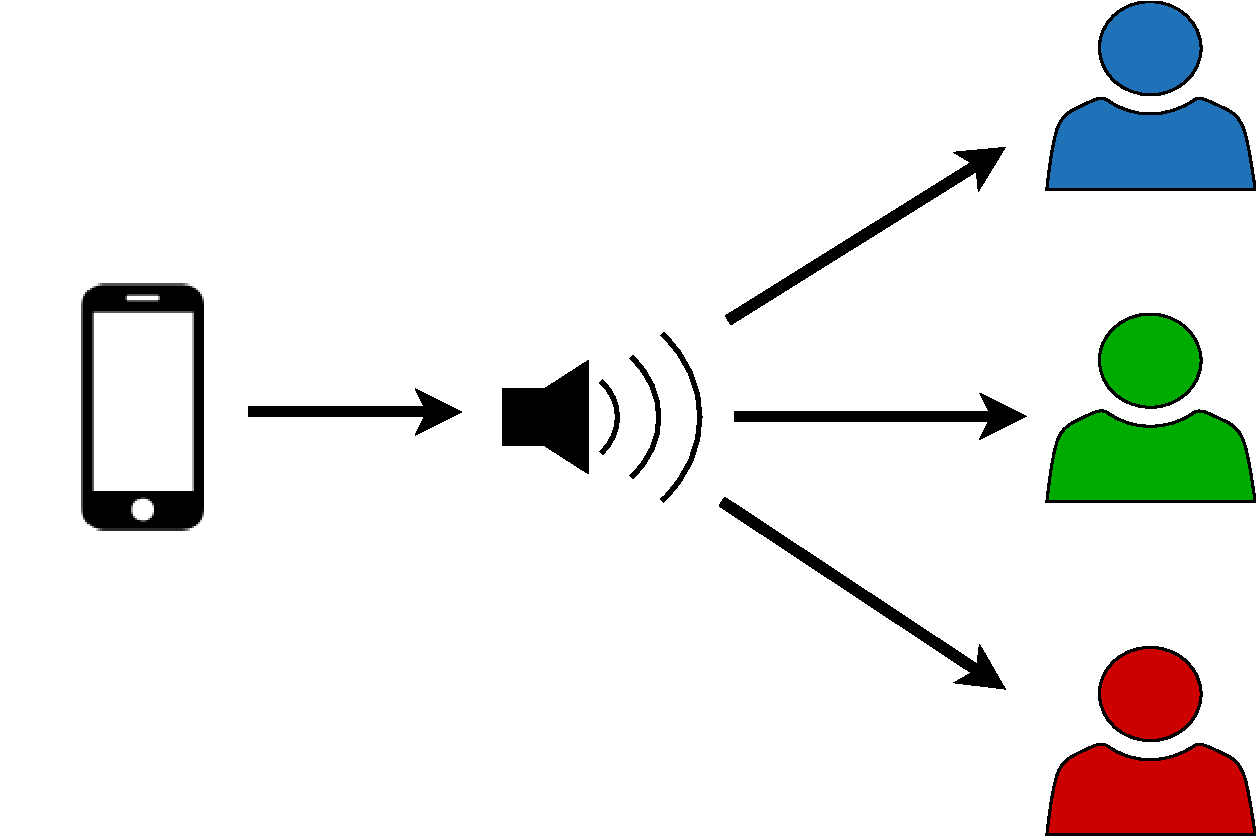
\includegraphics[width=0.45\textwidth]{speech_no_adapt}
		\label{fig:output_not_adapted}} 
	\hfill % no empty line here to avoid staring a new paragraph (figures will be vertically aligned)
	\subfigure
		[An illustration of a device's output, which is \emph{personalized} for each user.
		A different, customized spoken output (in blue, green, and red) is played to each user.]
		{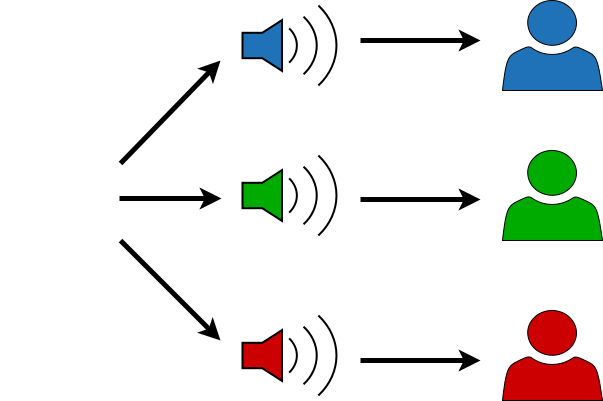
\includegraphics[width=0.45\textwidth]{speech_adapt}
		\label{fig:output_adapted}}
	\caption[Static vs.\ adaptive speech output]
		{Schematic comparison between an interaction with static spoken outputs (on the left) and an interaction with adaptive (i.e., personalized) spoken outputs (on the right).
		The system that adapts to the user makes the interaction tailored to the user's behavior.}
	\label{fig:static_vs_adaptive_speech_output}
\end{figure}

Dynamically changing the voice is a capability currently ascribed almost exclusively to humans and exist only sparsely and simplistically in computer-based systems.
A voice-activated device always talks the same way, regardless of how the user speaks to it, the environment and setting in which the interaction takes place, the goal and role of the device, etc.
This capability, which comes naturally to humans in social interactions, involves several steps of (partially unaware) decisions, which together form the overall effect of becoming behaviorally more or less similar to an interlocutor, as explained in \cref{sec:communication_accommodation_theory}.
These include both situational and knowledge-related facets like how it is expected to behave in certain situations and which vocal changes fit those, as well as the physiological ability to apply these matches.
Humans can perform all of these steps as one conduct.
For computers, however, these steps must be broken down and \emph{explained}, as they lack such common social background knowledge and the intuition as for how to match their voice to the situation.
Several attempts to integrate this capability into \acp{sds} are presented below, followed by a description of a roadmap toward such a system and an introduction of relevant terminology to describe these different steps and ways to achieve accommodative vocal behavior in machines.
The parallelisms to the human perspective are highlighted along the way to help to understand the motivations and goals.

\todo[inline]{here take 2-3 systems (from Chapter 1 and/or 3) and explain a bit in detail how they implemented the accommodation capabilities. specifically, emphasize the limitations and hint how the work here is doing more}

\citet{Bernsen1998designing}
\todo[inline]{this book (which I have) has a broad and detailed information about this topic. can take some hints from there}

\todo[inline]{say that, with current technology, only the user can vocally accommodate to the system, which is different from the HHI case.}

%Studying convergence in speech in an \ac{hci} context is made possible with more natural synthesis technology, which gives more fine-grained control over parameters of the system's spoken output.

% A technical overview of the development of adaptive \acp{sds} is given by \citet{Levitan2016implementing}, where speech rate and intensity are entrained by the system.

\subsection{Roadmap and challenges}
\label{subsec:roadmap_and_challenges}

\subsubsection{Dialogue is hard}
\label{subsubsec:dialogue_is_hard}

\citep{Turing1950computing}\ldots
\todo[inline]{points from Milica's slides}

\subsubsection{Suggested roadmap}
\label{subsubsec:suggested roadmap}

The lack of accommodative speech in computer-based systems roots from what is more often than not natural and even automatic for humans, namely realizing how and how much to change their vocal behavior, the physiological means to express those differences, and the ability to combine the two into a coherent production in an interaction.
\Cref{fig:roadmap_adaptive_sds} shows an overview of a (simplified) roadmap to integrating adaptive capabilities into a \ac{sds}.
In addition to the expected functionalities of a standard \ac{sds}, three main elements are required:
For one thing, knowledge about the nature and properties of accommodative behaviors in humans is required.
This includes both empiric experimental data and integrable models.
% 1-2 sentence that at the moment there are many ways to measure accommodation and existing models are limited (reference? or at least point to terminology part)
Furthermore, the technical capability to control the speech output on demand is essential for introducing flexibility in the system's base voice.
This also includes a mechanism for accumulating phonetic evidence from the user's input relevant for the feature representations used for the accommodation process.
As these manipulations must be applied in real-time, re-training the \ac{tts} model to capture every change is not only insufficient, but not practical as well.
This means that the manipulations are done on top of the existing \ac{tts} model, either by modifying the outputted waveform directly or by training a model that can take specific changes in feature description into consideration.
\putref{if chapter about those methods comes to life, refer to them}
To link between the modeled theoretical knowledge and the audio processing engineering implementations, an additional component must be introduced in the system.
The role of this component is to feed the system's flexible voice parameters result from the models to express vocal changes, which are ultimately conveyed to the user.
This emphasizes the notion of the \ac{nlg} module decides \emph{what} the system says while the \ac{tts} module determines \emph{how} it will say it.
This is further explained and illustrated in \cref{chap:convergence_module_for_sdss,fig:adaptation_module_architecture}.

This work addresses each of those facets.
\putref{when parts are more final, briefly refer to them here}
These aspects make the task of integrating flexible vocal characteristics into \acp{sds} an involved task, each with its own challenges that requires a profound work to investigate.
%
\begin{figure}[t]
	\centering
	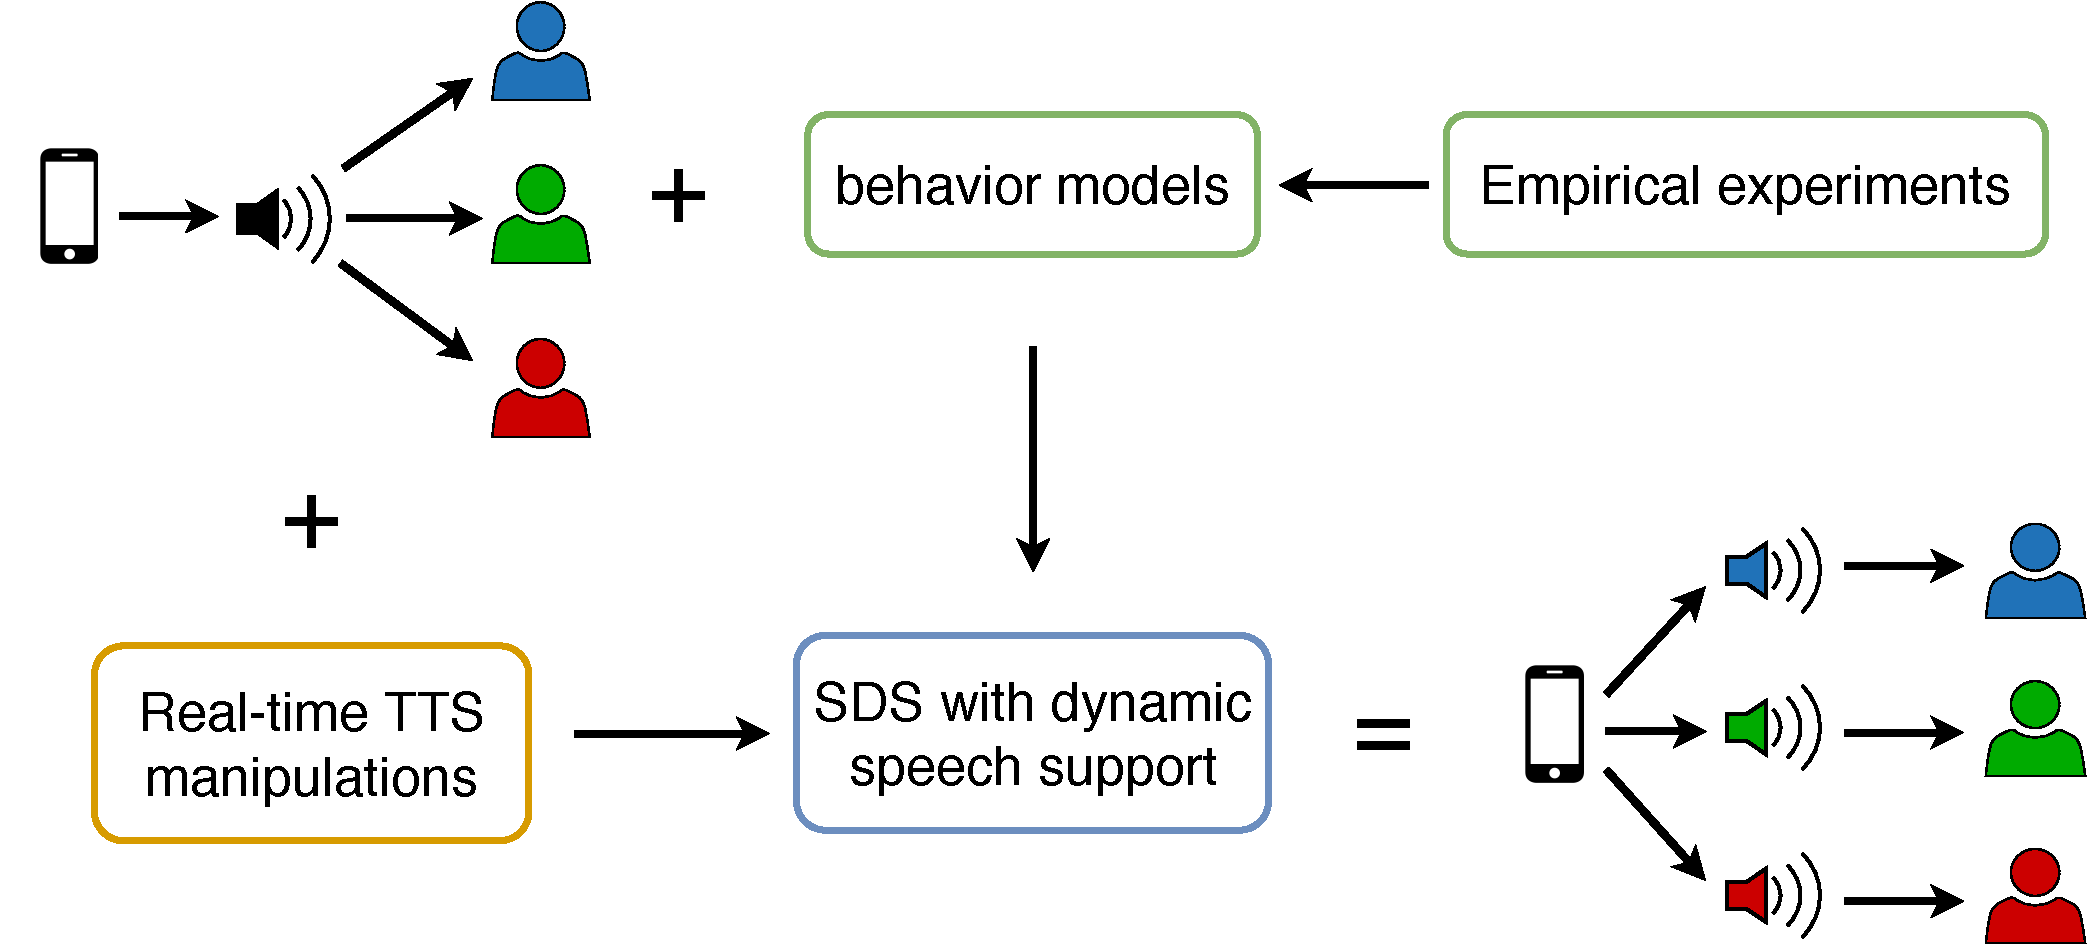
\includegraphics[width=\linewidth]{roadmap_adaptive_sds}
	\caption[Roadmap to phonetically adaptive \acl{sds}]
		{A suggested roadmap from static outputs (top left) to personalized outputs (bottom right) in \acp{sds} (and see \cref{fig:output_not_adapted,fig:output_adapted}).
		The green, orange, and blue blocks stand for the modeling, manipulation, and integration components described in the text, respectively.
		The \enquote*{+} signs represent direct addition to a static system and the arrows go from components required as a feed to others.}
	\label{fig:roadmap_adaptive_sds}
\end{figure}
%
For a \ac{sds} to accommodate with its speech, it would not only need to support dynamic, on-demand changes of its \ac{tts} component's output, but would also need its \ac{asr} component to be able to identify and track specific features in the user's speech to update its representation of those features.
Completing the cycle, these representations can then be used as additional input for the \ac{tts} components to determine how those would influence the system's speech output.
This process is individual for each speaker (see \cref{fig:static_vs_adaptive_speech_output}) and may occur over long periods of time or multiple interactions, depending on the desired degree and characteristics of accommodation.
Furthermore, this process may involve other components of the \ac{sds} as well (cf.\ \cref{fig:sds_architecture}).
For instance, the Dialogue Manager might consider changes in the user's speech when making decisions, e.g., based on apparent mood and calmness.
The \ac{nlg} component could make alterations to its output to better fit the vocal changes of the system and the user's dynamic state, such as shortening sentences and omit additional information if phonetic indicators of hurry or urgency (like those shown by \citet{Edworthy2003acoustic}) are detected in the speech input.

\subsection{Accommodation levels -- terminology}
\label{subsec:accommodation_levels}

In addition to all the above, another design choice for accommodative \acp{sds}, which is not explicitly required in human speech, concerns the overall \emph{level of accommodation} the system introduces.
This determines the fundamental behavior and form of variation in the system's speech, regardless of specific phonetic features, utterance contents, etc.
The variation levels (or properties) described below can potentially be combined in different ways to achieve the desired system behavior.
They are, at least to some extent, analogous to aforementioned processes conducted by humans in social interactions, with the key difference that humans don't need to defined and think about them separately, if at all.
The utilization of these levels is demonstrated in the context of phonetic accommodation, which is one case of dynamic change of speech \citep[as in][to name a few]{Weise2019individual, Schweitzer2016exemplar, Bevnuvs2014social}.
\Cref{chap:web-based_responsive_spoken_dialogue_system} further discusses and demonstrates the integration of such properties into a \ac{sds}.

Different terms are used in the literature to describe systems that can change their output.
This often leads to inconsistencies and mix-ups in terminology.
Definitions of five core properties of accommodative \ac{tts} that should, once accomplished, grant a more dynamic appearance, along with their suggested use and potential fusion with one another, are suggested below.
These terms seek to distinguish between the different capabilities that can be integrated into \acp{sds} and the way they relate to humans’ behaviors and each other.
%
\begin{description}
	\item[Adaptive] -- the vocal behavior evolves between and/or during interactions.\\
	This property refers to the system's use of any mean to \emph{dynamically} change it speech-related behavior, regardless of the source of influence, the goal or direction, or specific realizations.
%	Here, adapting means shifting the overall behaviors by updating a subset of the other properties.
	That means, for example, modifying the base behavior, extending the variability, or reflecting the system's changes earlier.
	This can happen between interactions or within a single, usually longer, interaction.
	The former could be more useful for \ac{cnc} systems or goal-oriented \acp{sds} that are used by many users, while the latter is more suitable for social systems like chatbots and \acp{pa} (see \cref{sec:types_of_sdss}).
	Ultimately, this is a means for the system to improve its performance and accessibility based on previous interactions.
	However, for some applications, like a \ac{capt} system, for example, it would be better to \enquote{reset} their behavior between each use to offer a better experience.

	\item[Flexible] -- on-demand speech manipulation \emph{without rebuilding the voice}.\\
	This property refers to the \emph{technical capability} to alter the system's speech output on request, which is achieved either via modifications in the voice's representation and parameters or by manipulating the outputted waveform directly using signal processing methods.
	Note that this does not entail the way this capability is used, and especially not that it is applied automatically.
	Moreover, as mentioned above, the technical capability to control the voice alone is not enough to create an accommodative behavior.
	This would also require additional data to be transferred to the \ac{tts} component to determine what manipulation to perform.
	For that end, the modeling steps can be built on top of this technical ground.
	It is important to note that this property compensates for the inherent ability in humans to control their voice at will, and therefore does not directly represent any specific element of humans' speech behavior like the other properties.
	
	\item[Responsive] -- changes are influenced by some \emph{external} speech input.\\
	A responsive system can, for instance, detect some target features in the user's speech input and, after comparing them to the system's representation of these features, guide the \ac{tts} on how to update them (typically, to make them more similar to the user's input).
	This requires a computational model that performs these steps (cf.\ \cref{chap:computational_model}).
	Yet this model would not have an independently defined behavior and it could only directly become more similar (or dissimilar) to the user in some fashion.
	Such models can be designed to imitate the user's immediate output from previous turns (like in \citet{Levitan2016implementing}) or to gradually match it based on some parameters like sensitivity and interaction's history (as demonstrated in \citet{Raveh2017Interspeech}).
	This property represents the idea that humans change their speech (and behavior in general) when interacting with other people, which is a key aspect of the \ac{cat} \citep[][and see \cref{sec:communication_accommodation_theory}]{Giles1991CAT}.
	
	\item[Characterized (Profiled)] -- the system's voice has its own base behavior.\\
	Giving a \enquote{character} (or a \emph{profile}) to a voice means that it has a specified base behavior, which might include general properties of accommodation.
	This can also be seen as a \emph{role} the system plays in a conversation, e.g., if built based on a certain \ac{hhi} scenario \citep{Silber-Varod2018prosodic}.
	In that case, the system would try to stick to some pre-defined model, which contains the required information to fulfill said role.
	A system might also have several profiles to switch between based on the settings and goals of the interaction.
	In the context of accommodation, that would include, for example, the degree of accommodation, its timing, or how strongly the system will try to influence the user's speech.
	This property represents the fact that a human being has a certain -- however complex -- personality.
	More specifically, a vocal identity, which will be expressed in spoken interactions.
	This idea is the basis for the simulations presented \cref{chap:statistical_model}, where each generative model can be seen as a core behavior.
	
	\item[Variable] -- variations on top of the base behavior are yielded.\\
	Some variations can be introduced based on the base profile.
	These are relatively minor differences that deviate from the voice's characteristics or enhance them in some way.
	From a system's point of view, the main purpose of such variations is to make the output style non-deterministic and therefore less repetitive and predictable.
	From the human point of view, this coincides with the difficulty to reproduce identical utterances in exactly the same way every time.
	Moreover, people, though having their own individual personality, would speak differently based on various factors outside a conversation like their mood, the environmental conditions, time constraints, etc.
	This property comes, therefore, to grant some smaller-scale dynamics to the voice, in particular when its base behavior is deterministic.
	\Cref{chap:statistical_model} explains in details an approach to achieve such variational behaviors with examples provided in \cref{sec:clustering_and_incremental_generation,tab:generated_symbol_sequences}.
\end{description}
%

% ----------
% REVIEW: Only mention in case some statistical model is include in the thesis that deals with that (a time-series one or variational autoencoder). in that case briefly say what it means and refer to the relevant chapter

%This work concentrates on facets concerning the properties \emph{characterized} and \emph{variable}, which have been given little attention in \ac{sds} research.
%Together, these two properties results in a flexible, non-deterministic output derived from a defined core behavior (that might itself vary).
%Added to the responsive output creates a system that changes with respect to the user according to its own base behavior and probabilistic variations.
%The balance between the influences from the user input and the system's profile can be defined as well, similarly to the bias utilized in speech adaptation, in the form of \putref{reference to this method)}
%\todo{sentence about balance might be unnecessary}
% ----------

\subsection{Systems with accommodation capabilities}
\label{subsec:systems_with_accommodation_capabilities}

\citet{Levitan2016implementing} % the system that (linearly?) entraining. read the deatils again and then say how this differs from the architecture in this paper. also, find references there for more such systems.

\section{Evaluating spoken dialogue systems}
\label{sec:evaluation_of_sdss}

\todo[inline]{decide whether a section about evaluation is necessary}

\ldots Therefore, evaluation of \acp{sds} depends on the purpose of the systems, which can be divided into two types, namely \textit{\aclp{tds}} and \textit{\aclp{ngs}}.

\subsection{Task-driven Systems}
\label{subsec:task-driven_systems}
[doesn't really evaluate the \ac{sds}, but it's ability to predict what task should be performed]
[typically part of a bigger system (which has a set of tasks it can perform (e.g. personal assistant))]

\subsection{Non-goal Systems}
\label{subsec:non-goal_systems}

A \acf{ngs} is a \ac{sds} that does not necessarily aim to complete a specific task (unlike \acp{tds}).
Its purpose is, then, more general and there might not even be a defined purpose for it.
Chatbots (see \cref{subsec:chatbots}) are a good a example for a \ac{sds} that typically isn't used for accomplishing a practical task like getting information or operating a device.
Instead, they are used as a long-term social companion (be it at home or as part of a mobile device) and even merely for entertainment. \todo{references for both examples}
Since such systems don't help to achieve a defined goal, it is not possible to evaluate their performance based on how well (or whether at all) this goal task was carried out.
There is a need therefore for another, more long-term and interaction-oriented method rather than a task-oriented method.
On the one hand, from the \ac{hci} point of view, the advantage of such methods is that they evaluate the dialogue capabilities of the system and not merely it's ability to map speech patterns or keywords to a set pre-defined actions.
On the other hand, however, the problem in such methods is that it is much harder to define metrics when the goal of the interaction is not completely defined.
There are two approaches to solve this issue:
The first is defining the 
